\documentclass[runningheads]{llncs}

\usepackage[T1]{fontenc}
\usepackage{graphicx}
\usepackage{hyperref}
\usepackage{color}
\usepackage{listings}
\usepackage{booktabs}
\usepackage{amssymb}
\usepackage{xspace}
\usepackage{tikz}
\usepackage{tcolorbox}
\usetikzlibrary{positioning, arrows.meta}
\renewcommand\UrlFont{\color{blue}\rmfamily}

\newcommand{\sysname}{CyberGraph\xspace}

\lstset{
  basicstyle=\ttfamily\scriptsize,
  breaklines=true,
  frame=single,
  language=SQL,
  morekeywords={MATCH,RETURN,WHERE,ORDER,BY,OPTIONAL,AS,IN,nodes,length,path},
  keywordstyle=\bfseries,
  commentstyle=\itshape\color{gray},
  showstringspaces=false,
  aboveskip=2pt,
  belowskip=2pt
}

\begin{document}

\title{\sysname: A Demo of Conversational Threat Analysis for Web Infrastructure with Knowledge Graphs}
\titlerunning{\sysname: Conversational Threat Analysis Demo}

\author{First Author\inst{1} \and
Second Author\inst{1} \and
Third Author\inst{1}}
\authorrunning{F. Author et al.}

\institute{Institute of Computer Science, University, City, Country \\
\email{first@example.edu, second@example.edu, third@example.edu}}

\maketitle

\begin{abstract}
Modern web infrastructures are increasingly difficult to inspect and protect because vulnerability impact propagates through layered dependencies across services, libraries, and hosts. At the same time, recent advances in conversational and agentic systems create new opportunities to support security operations through natural-language interaction rather than manual cross-tool inspection. This paper presents \sysname, a working demo of an agentic conversational system for threat analysis over web infrastructure represented as a property graph in Neo4j. Given an operator question, \sysname translates the request into Cypher, retrieves affected services together with explicit dependency paths, and can then orchestrate a remediation workflow after human confirmation. The novelty of the demo lies in unifying conversational querying, graph-grounded impact tracing, and confirmation-gated response execution within a single end-to-end interaction loop. The paper describes the system architecture, the live demonstration scenario, and the current implementation status.

\keywords{Knowledge Graph \and Web Security \and Neo4j \and Conversational Systems \and Demo}
\end{abstract}

\section{Introduction}
Recent high-impact vulnerabilities such as Log4Shell~\cite{cve2021log4shell} have shown that a single flawed library may propagate risk across numerous dependent services in a modern web stack. In operational practice, however, identifying a vulnerable component is only the beginning. Operators must still determine which user-facing services are exposed through dependency chains, what evidence supports that assessment, and which remediation actions should be prioritized. This process remains cumbersome in microservice-based environments, where service relationships, deployment information, and vulnerability data are distributed across multiple tools and administrative views.

Meanwhile, conversational and agentic interfaces are beginning to reshape how complex web systems are inspected and managed. Rather than requiring operators to manually navigate dashboards, logs, and dependency inventories, such interfaces can support a more direct interaction style in which high-level questions are translated into grounded system analyses. For security-sensitive tasks, however, such interaction must remain explainable, evidence-based, and subject to human control.

\sysname is designed to explore this opportunity through an interactive demo for conversational threat analysis over web infrastructure. The system represents infrastructure entities and their security relations as a graph, accepts natural-language questions, translates them into Cypher, and returns affected services together with explicit dependency chains. When a high-risk condition is identified, the prototype can further invoke a remediation workflow after explicit operator confirmation. In this sense, \sysname is not merely a text-to-query interface; it is a compact agentic workflow that connects conversational intent, graph-grounded analysis, and human-supervised action.

The novelty of the demo lies in the integration of three capabilities within a single end-to-end interaction loop: (i) conversational querying for vulnerability impact inspection, (ii) graph-based tracing that exposes explicit dependency evidence, and (iii) confirmation-gated workflow execution that links analysis to operational response. This setting aligns well with the ICWE 2026 theme on agentic and autonomous web systems, particularly with respect to security, trust, and conversational interfaces.

This demo paper focuses on the running system, the end-to-end interaction loop, and the concrete live demonstration scenario. The prototype brings together ideas from graph-based security analysis~\cite{peng2022threat,li2024graphrag}, natural-language query generation~\cite{chen2023text,gao2023texttosql}, and security orchestration~\cite{islam2023soar,milajerdi2019holmes} within a unified workflow suitable for a live conference demonstration.

\section{System Overview}
\begin{figure}[t]
\centering
\resizebox{0.96\columnwidth}{!}{%
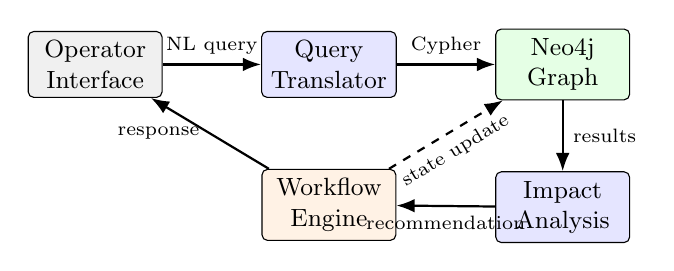
\begin{tikzpicture}[
    node distance=0.8cm and 1.25cm,
    >=Latex,
    box/.style={draw, rounded corners=2pt, minimum width=1.7cm, minimum height=0.72cm, align=center, font=\small},
    userbox/.style={box, fill=gray!12},
    llmbox/.style={box, fill=blue!10},
    dbbox/.style={box, fill=green!10},
    actbox/.style={box, fill=orange!10},
    arrow/.style={->, thick},
    lbl/.style={font=\scriptsize, midway}
]
\node[userbox] (user) {Operator\\Interface};
\node[llmbox, right=of user] (translator) {Query\\Translator};
\node[dbbox, right=of translator] (graph) {Neo4j\\Graph};
\node[llmbox, below=0.9cm of graph] (analysis) {Impact\\Analysis};
\node[actbox, below=0.9cm of translator] (workflow) {Workflow\\Engine};
\draw[arrow] (user) -- node[lbl, above] {NL query} (translator);
\draw[arrow] (translator) -- node[lbl, above] {Cypher} (graph);
\draw[arrow] (graph) -- node[lbl, right] {results} (analysis);
\draw[arrow] (analysis) -- node[lbl, below] {recommendation} (workflow);
\draw[arrow] (workflow) -- node[lbl, left] {response} (user);
\draw[arrow, dashed] (workflow) -- node[lbl, below, sloped] {state update} (graph);
\end{tikzpicture}%
}
\caption{Overview of \sysname. A natural-language security query is translated into Cypher, executed on the infrastructure graph, and linked to an optional remediation workflow.}
\label{fig:arch}
\end{figure}


\textbf{Infrastructure graph.}
The system models servers, microservices, libraries, and CVEs in Neo4j~\cite{robinson2015graph}. In the current prototype, four node types are employed: \texttt{Server}, \texttt{Microservice}, \texttt{Library}, and \texttt{CVE}. The graph captures hosting relations, inter-service and service-to-library dependencies, as well as vulnerability links.

\textbf{Conversational query translation.}
A large language model receives a schema-aware prompt and translates natural-language security questions into read-only Cypher queries. This component serves as the conversational front end of the system, allowing operators to express analytical intent at a high level rather than through handcrafted graph queries. The prompt includes the graph schema, safety constraints, and representative query patterns for impact analysis, dependency inspection, and blast-radius exploration.

\textbf{Graph-grounded impact analysis.}
The generated Cypher is executed on the graph to identify affected services and their corresponding dependency paths. In the current prototype, bounded traversal over vulnerability and dependency edges is employed to support efficient impact tracing. This design keeps the conversational interaction grounded in explicit graph evidence, thereby making the returned answers more interpretable during live use. A representative query is shown below.

\begin{lstlisting}
MATCH path = (cve:CVE {id: $cveId})
  <-[:HAS_VULNERABILITY]-(lib:Library)
  <-[:DEPENDS_ON*1..5]-(svc:Microservice)
RETURN svc.name AS service,
       length(path) AS depth,
       [n IN nodes(path) | n.name] AS chain
ORDER BY depth
\end{lstlisting}

\textbf{Confirmation-gated workflow execution.}
When the analysis indicates a critical case, the system can invoke an n8n-based workflow engine to perform a predefined response action. In the current implementation, such an action is executed only after explicit operator confirmation, thereby preserving human oversight. This mechanism allows the demo to illustrate an agentic interaction pattern without removing the operator from the decision loop.

\section{Demonstration Scenario}
\begin{figure}[t]
\centering
\begin{tcolorbox}[
  colback=gray!3,
  colframe=gray!55,
  fontupper=\scriptsize\ttfamily,
  boxrule=0.5pt,
  arc=2pt,
  left=3pt, right=3pt, top=2pt, bottom=2pt,
  title={\scriptsize\sffamily Demo Scenario: Log4Shell},
  fonttitle=\bfseries\scriptsize\sffamily
]
\textbf{Operator:} Which services are affected by Log4Shell?\\[2pt]
\textbf{System:} Querying the infrastructure graph.\\[2pt]
{\color{red}\textbf{Result:}} 4 affected services for \texttt{CVE-2021-44228}.\\[2pt]
\textbf{Affected services:}\\
\hspace*{0.5em}\textbullet\ \texttt{payment-service} (PCI), direct dependency on \texttt{log4j-core}\\
\hspace*{0.5em}\textbullet\ \texttt{notification-service}, direct dependency on \texttt{log4j-core}\\
\hspace*{0.5em}\textbullet\ \texttt{auth-service}, reachable in 2 hops\\
\hspace*{0.5em}\textbullet\ \texttt{user-portal}, reachable in 3 hops\\[2pt]
\textbf{System:} Recommended action: isolate \texttt{payment-service}.\\[2pt]
\textbf{Operator:} Confirm isolation.\\[2pt]
\textbf{System:} Action executed. Service state updated to \texttt{quarantined}.
\end{tcolorbox}
\caption{Compact interaction shown during the live demo.}
\label{fig:demo}
\end{figure}


The demo is designed to be concise, repeatable, and interactive. It can be completed within a few minutes and readily repeated for different attendees. The primary scenario is centered on the Log4Shell vulnerability.

\textbf{Step 1: present the infrastructure view.}
The presenter first introduces a graph containing 3 servers, 5 microservices, 4 libraries, and 2 CVEs. Both direct service-to-library dependencies and transitive service-to-service dependencies are visualized for the audience.

\textbf{Step 2: issue a natural-language query.}
A participant then poses a question such as \emph{``Which services are affected by Log4Shell?''} The system displays the generated Cypher and executes it against Neo4j.

\textbf{Step 3: inspect the analysis result.}
The interface returns the affected services, hop distance, and dependency paths. In the current example, \texttt{payment-service} and \texttt{notification-service} are directly affected, whereas \texttt{auth-service} and \texttt{user-portal} are exposed through transitive paths.

\textbf{Step 4: confirm a response action.}
If the result indicates a severe condition, the system recommends a remediation step. The operator may then confirm a predefined action, such as isolating \texttt{payment-service}.

\textbf{Step 5: observe the updated state.}
After confirmation, the workflow engine applies the response action and the graph state is updated accordingly. The audience can immediately observe both the executed action and the resulting system status.

This scenario is well suited to the ICWE demo track because it makes the artifact, the conversational interaction flow, and the human-in-the-loop agentic experience concrete and directly observable.

\section{Implementation and Current Status}
The prototype integrates Neo4j for graph storage, an LLM-based text-to-Cypher module, and n8n for workflow execution. The current implementation supports graph initialization, read-only Cypher generation, impact analysis, blast-radius inspection, and a simple remediation path in which a service is marked as quarantined after operator confirmation.

The demo dataset is intentionally compact so that the full interaction remains understandable in a live presentation setting. It includes two representative vulnerabilities, Log4Shell and Spring4Shell, together with a dependency structure that makes transitive impact readily visible. The implementation further includes benchmark queries and automated tests for graph setup, query execution, and remediation logic.

At the current stage, the prototype should be understood as a research demo rather than a production-ready security platform. The objective of the live presentation is to demonstrate that an agentic conversational interface can assist operators in inspecting vulnerability impact over a graph-based representation of web infrastructure and in connecting such analysis to concrete, human-supervised response actions.

\section{Conclusion}
\sysname demonstrates that knowledge graphs, conversational interfaces, and workflow execution can be combined into a compact agentic web-security artifact for threat analysis. The system enables operators to move from a vulnerability identifier to affected services, explicit dependency paths, and a confirmed response within a single interaction loop. More broadly, the demo suggests that conversational and agentic system designs provide a promising interface paradigm for explainable, human-in-the-loop security operations over complex web infrastructures.

\paragraph{Generative AI Disclosure.}
The authors used generative AI tools to assist with language editing and manuscript revision. All technical content, system design decisions, experimental claims, and final wording were reviewed and verified by the authors.

\bibliographystyle{splncs04}
\bibliography{references}

\end{document}
